\documentclass[dvipdfmx,12pt,notheorems]{beamer}
%%%% 和文用 %%%%%
\usepackage{bxdpx-beamer}
\usepackage{pxjahyper}
\usepackage{minijs}%和文用
\usepackage{latexsym}
\usepackage{tikz}
\usetikzlibrary{calc,quotes,positioning}
\renewcommand{\kanjifamilydefault}{\gtdefault}%和文用

%%%% スライドの見た目 %%%%%
\usetheme{Madrid}
\usefonttheme{professionalfonts}
\setbeamertemplate{frametitle}[default][center]
\setbeamertemplate{navigation symbols}{}
\setbeamercovered{transparent=0}%好みに応じてどうぞ)
\setbeamertemplate{footline}[page number]
\setbeamerfont{footline}{size=\normalsize,series=\bfseries}
\setbeamercolor{footline}{fg=black,bg=black}
%%%%

%%%% 定義環境 %%%%%
\usepackage{amsmath,amssymb}
\usepackage{amsthm}
\theoremstyle{definition}
\newtheorem{theorem}{定理}
\newtheorem{definition}{定義}
\newtheorem{proposition}{命題}
\newtheorem{lemma}{補題}
\newtheorem{corollary}{系}
\newtheorem{conjecture}{予想}
\newtheorem*{remark}{Remark}
\renewcommand{\proofname}{}
%%%%%%%%%

%%%%% フォント基本設定 %%%%%
\usepackage[T1]{fontenc}%8bit フォント
\usepackage{textcomp}%欧文フォントの追加
\usepackage[utf8]{inputenc}%文字コードをUTF-8
\usepackage{otf}%otfパッケージ
\usepackage{txfonts}%数式・英文ローマン体を txfont にする
\usepackage{bm}%数式太字
%%%%%%%%%%

\newcommand{\func}[1]{\ensuremath\mathrm{#1}}
 
\title[略タイトル]{van Emde Boas Trees}
\author[Mitsuyoshi]{光吉 健汰}
\institute[IKN]{北海道大学工学部 情報エレクトロニクス学科 情報理工学コース 3年\\
	情報知識ネットワーク研究室}
\date{\today}%日付
\begin{document}

\begin{frame}[plain]\frametitle{}
\titlepage %表紙
\end{frame}

\begin{frame}\frametitle{Contents}
\tableofcontents %目次
\end{frame}

\section{van Emde Boas Trees とは}
\begin{frame}\frametitle{van Emde Boas Trees とは}
	van Emde Boas Treesは集合(set)以下の操作が可能なデータ構造
\begin{block}{操作}
\begin{description}
\setlength{\labelwidth}{15ex}
\setlength{\itemindent}{8ex}
\item[$\func{member}(e)$]		$e$が存在するかを返す\\
\item[$\min()$]			要素の最小値を返す\\
\item[$\max()$]			要素の最大値を返す\\
\item[$\func{succesor}(e)$]	$e$より大きい最小の要素を返す\\
\item[$\func{predecessor}(e)$]	$e$より小さい最大の要素を返す\\
\item[$\func{insert}(e)$]		$e$を挿入する\\
\item[$\func{delete}(e)$]		$e$を削除する\\
\end{description}
\end{block}
\begin{block}{}
\structure{これらの操作が最悪時間計算量$O(\log\log u)$で実行可能\\}
\end{block}
$u :=$ 保持できる要素の最大
\end{frame}

\section{配列での表現}
\begin{frame}\frametitle{配列での表現}
長さ$u$ のbit配列を確保し, 要素を持つならば, $1$を代入する. 
$S = { 0, 2, 5, 7}$
\begin{tikzpicture}[place/.style={rectangle,draw}]
	\node (0)[place]{0};
	\node (1)[place,right=of 0]{1};
	\node (2)[place,right=of 1]{2};
	\node (3)[place,right=of 0]{3};
	\node (4)[place,right=of 0]{4};
	\node (5)[place,right=of 0]{5};
	\node (6)[place,right=of 0]{6};
	\node (7)[place,right=of 0]{7};
\end{tikzpicture}
\end{frame}

\section{Segment Tree}
\begin{frame}\frametitle{まずは時間計算量$O(\log u)$を目指す}
\begin{itemize}
\item クエリ, 点更新を$O(\log u)$で行いたい
\item Segment Treeを使おう!
\begin{itemize}
\item 葉には$i$番目の要素が格納されているかを保存
\item 親のノードは子の論理和を格納
\end{itemize}
\end{itemize}
\onslide+<2->{\includegraphics[width=\textwidth]{segtree.eps}}
\end{frame}

\begin{frame}\frametitle{各種操作}
\begin{itemize}
\item $\func{member}(e)$は葉の$e$に該当するノードの値を返す
\end{itemize}
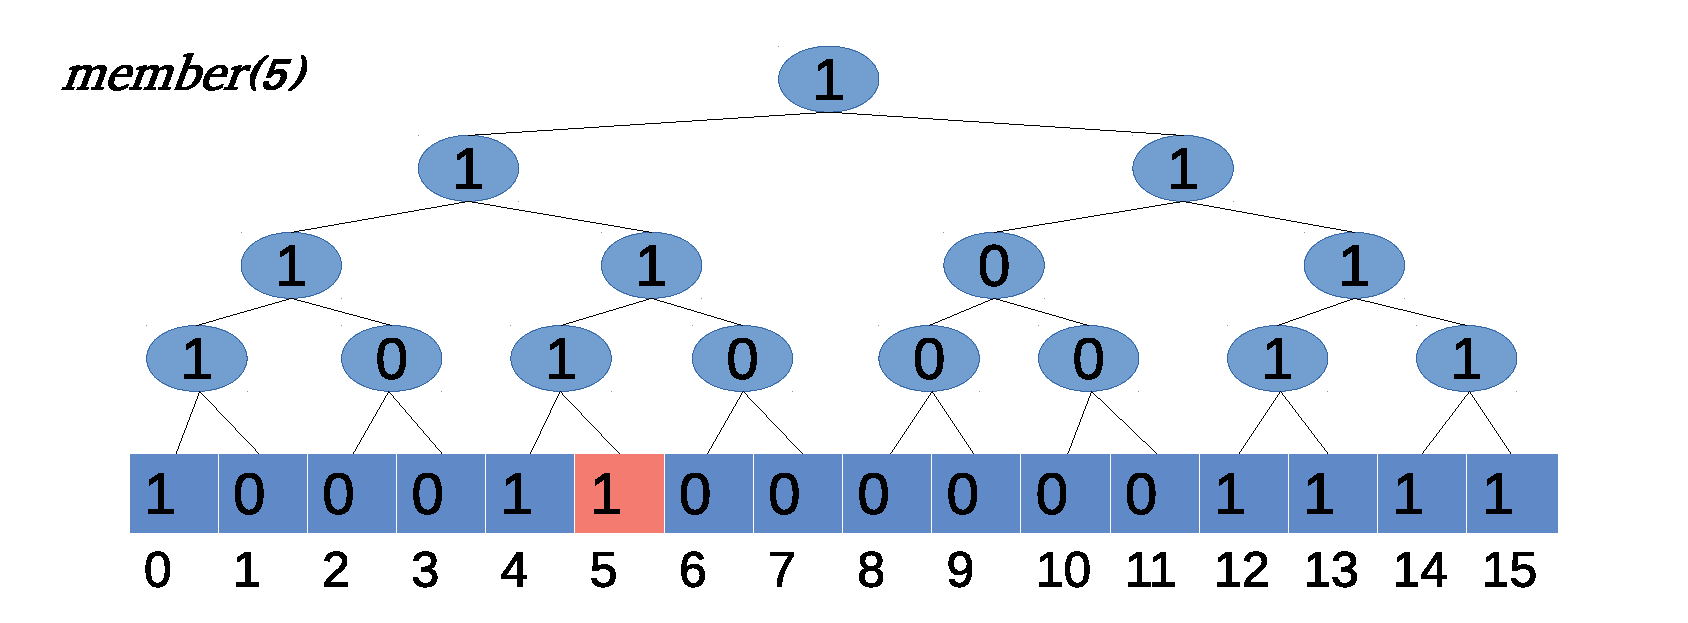
\includegraphics[width=\textwidth]{segtree_member.eps}
\end{frame}

\begin{frame}\frametitle{各種操作}
\begin{itemize}
\item $\min()$は$\func{successor}(-1)$として実行する
\item $\func{successor}(e)$は以下の処理を行う
\begin{itemize}
\item 親ノードからみて左の子, かつ右の子が$1$となるまで親のノードを上がり, 右の子に降りる
\item 左の子が$1$ならば左の子へ, そうでないならば右の子に降りる
\item 葉へ到達したらその葉の位置を返す
\end{itemize}
\item $\max()$, $\func{predecessor}(e)$も同様に行う
\end{itemize}
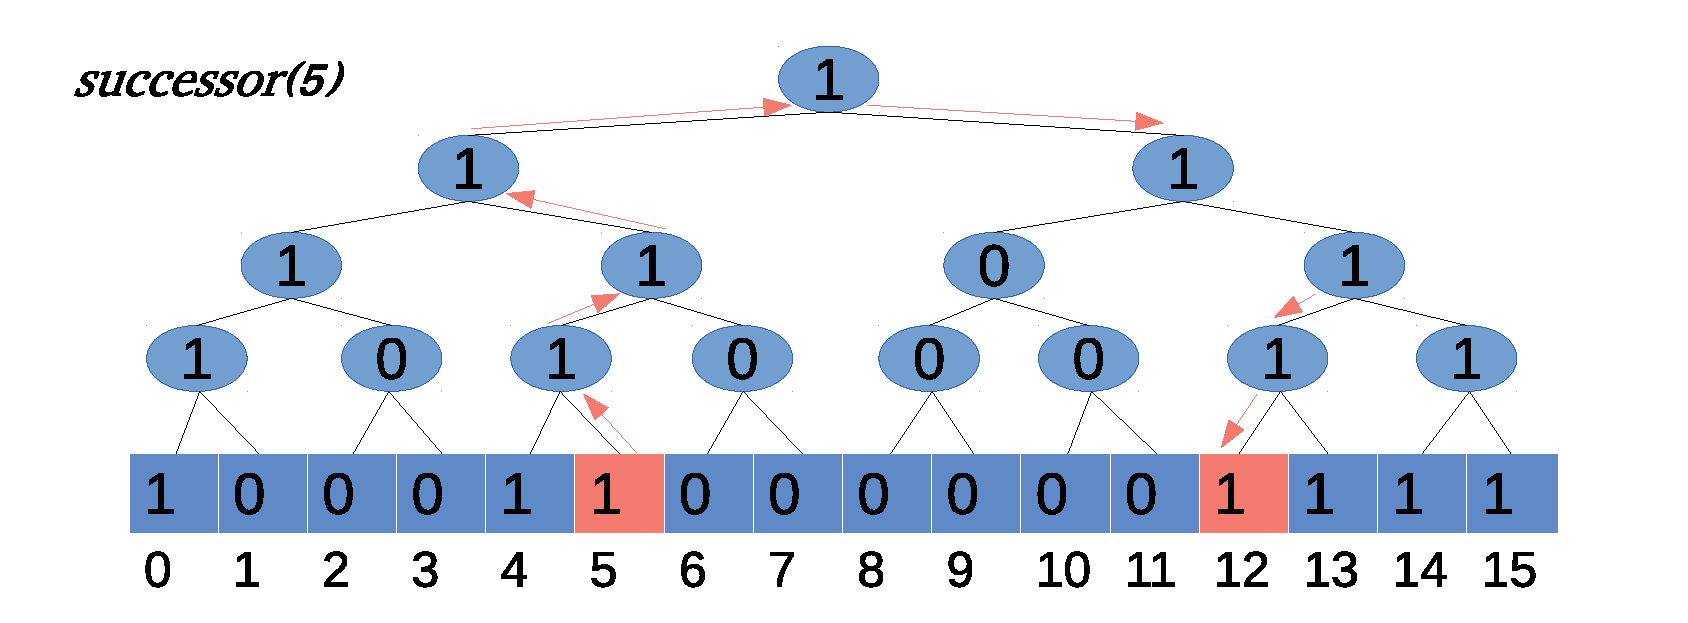
\includegraphics[width=\textwidth]{segtree_succ.eps}
\end{frame}

\begin{frame}\frametitle{各種操作}
\begin{itemize}
\item $\func{insert}(e)$は, 葉からノードの値を$1$にしながら親のノードへ上がる
\end{itemize}
\includegraphics[width=\textwidth]{segtree_insert.eps}
\end{frame}

\begin{frame}\frametitle{各種操作}
\begin{itemize}
\item $\func{insert}(e)$は, 葉からノードの値を$1$にしながら親のノードへ上がる
\end{itemize}
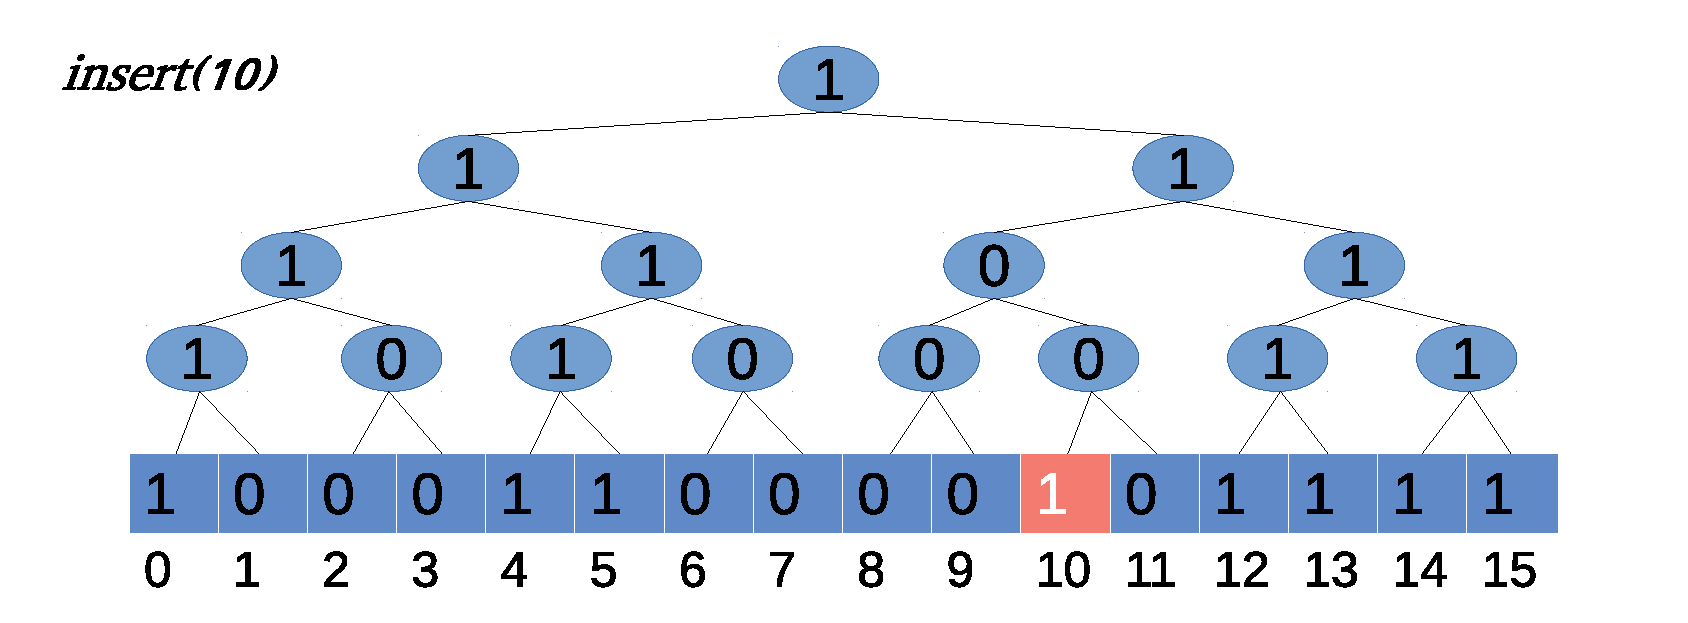
\includegraphics[width=\textwidth]{segtree_insert_0.eps}
\end{frame}

\begin{frame}\frametitle{各種操作}
\begin{itemize}
\item $\func{insert}(e)$は, 葉からノードの値を$1$にしながら親のノードへ上がる
\end{itemize}
\includegraphics[width=\textwidth]{segtree_insert_1.eps}
\end{frame}

\begin{frame}\frametitle{各種操作}
\begin{itemize}
\item $\func{insert}(e)$は, 葉からノードの値を$1$にしながら親のノードへ上がる
\end{itemize}
\includegraphics[width=\textwidth]{segtree_insert_2.eps}
\end{frame}

\begin{frame}\frametitle{各種操作}
\begin{itemize}
\item $\func{insert}(e)$は, 葉からノードの値を$1$にしながら親のノードへ上がる
\end{itemize}
\includegraphics[width=\textwidth]{segtree_insert_3.eps}
\end{frame}

\begin{frame}\frametitle{各種操作}
\begin{itemize}
\item $\func{delete}(e)$は, 以下の処理を行う
\begin{itemize}
\item 葉の値を$0$にし, 親のノードに上がる
\item 子が共に$0$ならば, 自身の値を$0$にし, 親のノードに上がる, そうでないならば処理を終了する
\end{itemize}
\end{itemize}
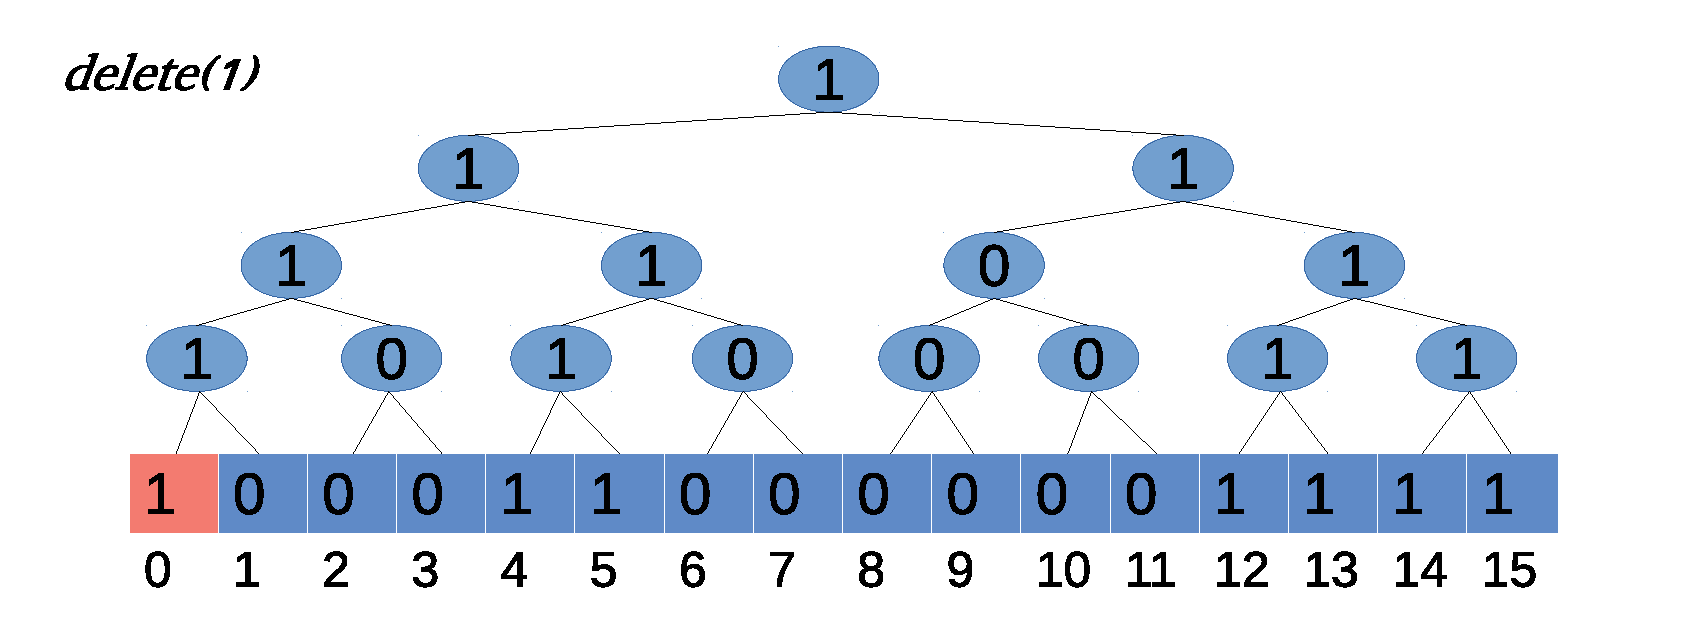
\includegraphics[width=\textwidth]{segtree_delete.eps}
\end{frame}

\begin{frame}\frametitle{各種操作}
\begin{itemize}
\item $delete(e)$は, 以下の処理を行う
\begin{itemize}
\item 葉の値を$0$にし, 親のノードに上がる
\item 子が共に$0$ならば, 自身の値を$0$にし, 親のノードに上がる, そうでないならば処理を終了する
\end{itemize}
\end{itemize}
\includegraphics[width=\textwidth]{segtree_delete_0.eps}
\end{frame}

\begin{frame}\frametitle{各種操作}
\begin{itemize}
\item $delete(e)$は, 以下の処理を行う
\begin{itemize}
\item 葉の値を$0$にし, 親のノードに上がる
\item 子が共に$0$ならば, 自身の値を$0$にし, 親のノードに上がる, そうでないならば処理を終了する
\end{itemize}
\end{itemize}
\includegraphics[width=\textwidth]{segtree_delete_1.eps}
\end{frame}

\begin{frame}\frametitle{各種操作}
\begin{itemize}
\item $delete(e)$は, 以下の処理を行う
\begin{itemize}
\item 葉の値を$0$にし, 親のノードに上がる
\item 子が共に$0$ならば, 自身の値を$0$にし, 親のノードに上がる, そうでないならば処理を終了する
\end{itemize}
\end{itemize}
\includegraphics[width=\textwidth]{segtree_delete_2.eps}
\end{frame}

\begin{frame}\frametitle{各種操作}
\begin{itemize}
\item $delete(e)$は, 以下の処理を行う
\begin{itemize}
\item 葉の値を$0$にし, 親のノードに上がる
\item 子が共に$0$ならば, 自身の値を$0$にし, 親のノードに上がる, そうでないならば処理を終了する
\end{itemize}
\end{itemize}
\includegraphics[width=\textwidth]{segtree_delete_3.eps}
\end{frame}

\begin{frame}\frametitle{各種操作}
\begin{itemize}
\item $delete(e)$は, 以下の処理を行う
\begin{itemize}
\item 葉の値を$0$にし, 親のノードに上がる
\item 子が共に$0$ならば, 自身の値を$0$にし, 親のノードに上がる, そうでないならば処理を終了する
\end{itemize}
\end{itemize}
\includegraphics[width=\textwidth]{segtree_delete_4.eps}
\end{frame}

\begin{frame}\frametitle{各種操作}
\begin{itemize}
\item $delete(e)$は, 以下の処理を行う
\begin{itemize}
\item 葉の値を$0$にし, 親のノードに上がる
\item 子が共に$0$ならば, 自身の値を$0$にし, 親のノードに上がる, そうでないならば処理を終了する
\end{itemize}
\end{itemize}
\includegraphics[width=\textwidth]{segtree_delete_5.eps}
\end{frame}

\begin{frame}\frametitle{計算量}
\begin{itemize}
\item \structure{空間計算量}
\par \hspace{1em} 葉の数は$u$個なので, ノードの合計数は$2u$個\\よって空間計算量は$O(u)$
\item \structure{時間計算量}
\par \hspace{1em} いずれの操作も, 1つのノードでの処理は$O(1)$\\どの操作も高々木の高さ($logu$)の2倍程度の数のノードに対し, 処理を行う, よって時間計算量は$O(2logu) = O(logu)$
\end{itemize}
\end{frame}

\begin{frame}\frametitle{どうやって高速化するか}
\begin{itemize}
\item Segment Treeでは木の高さが$logu$なので, 時間計算量も$O(logu)$に
\item<2-> 木の高さを小さくしよう!
\end{itemize}
\onslide+<2->{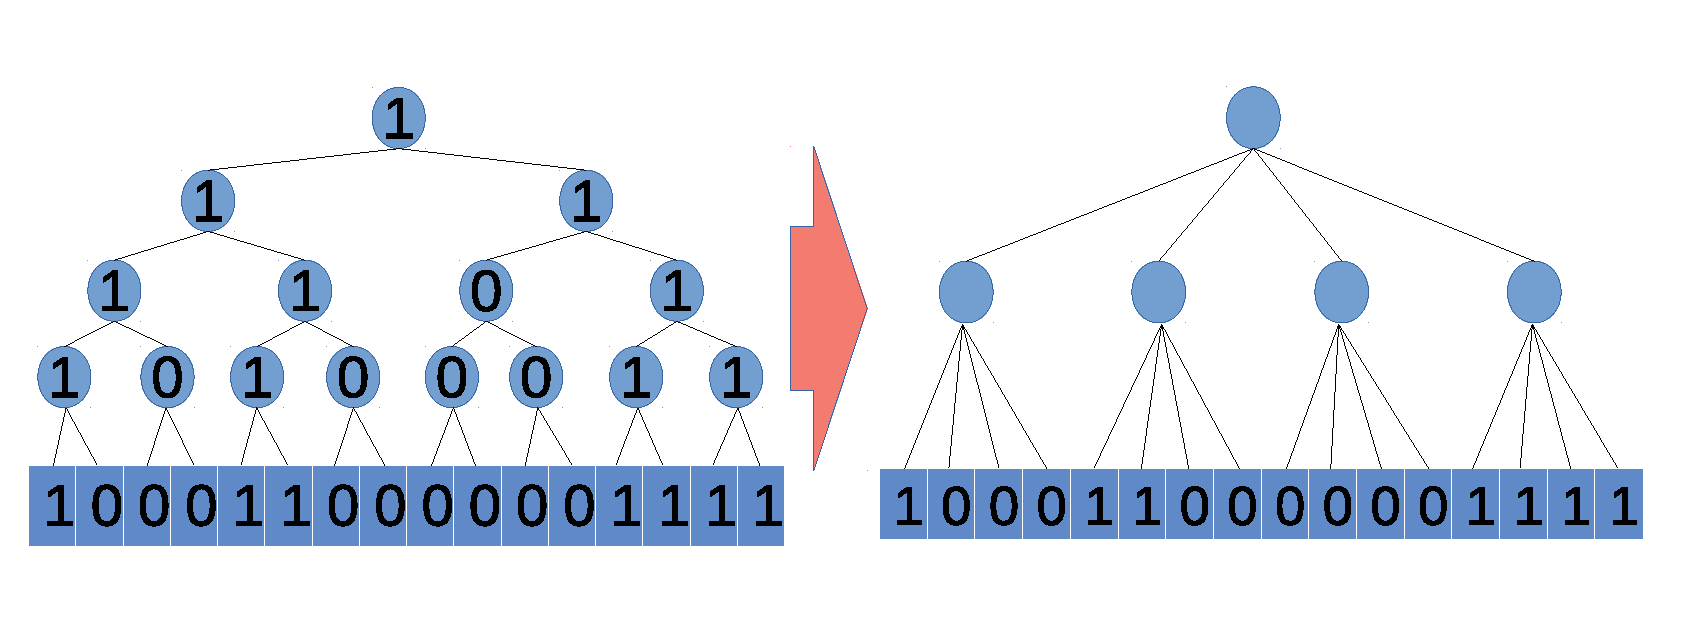
\includegraphics[width=\textwidth]{segtree_to_veb.eps}}
\end{frame}

\begin{frame}\frametitle{木を縮めるために}
\begin{itemize}
\item そのまま木の高さを小さくすることはできない
\pause
\item ノードが持つ情報を増やして木を縮めよう!
\end{itemize}
\begin{itemize}
\item 子のノードを, 自身のノード以下の葉の平方根の数だけ持つ
\begin{itemize}\item 子のノードのことを\structure{$cluster$}と呼ぶことにする\end{itemize}
\item 自身は, それぞれ子のノードが要素を持つかを保持しておく
\begin{itemize} \item これを\structure{$summary$}とする\end{itemize}p
\item 親のノードが持つ$cluster$の数は自身の持つ$cluster$の数の平方根となる$\rightarrow$木の高さは, \structure{$loglogu$}となる
\end{itemize}
\onslide+<2->{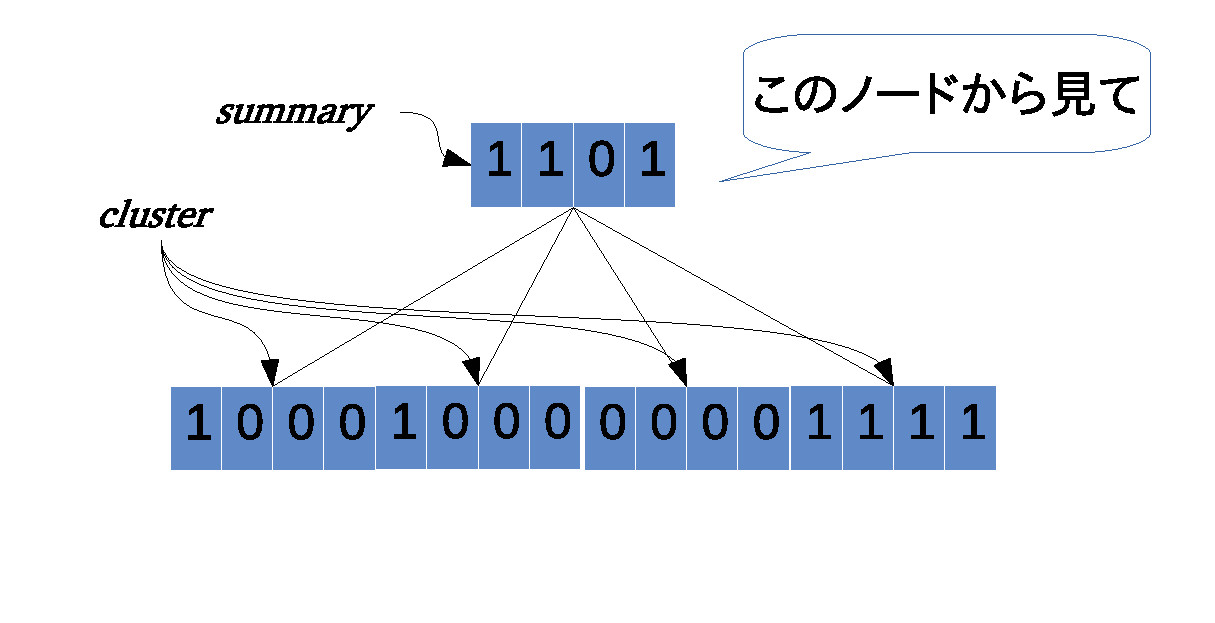
\includegraphics[width=0.75\textwidth]{veb_proto_abst.eps}}
\end{frame}

\begin{frame}{計算量はどう変わる?}
\begin{itemize}
\item このデータ構造でもSeg木同様, 完全二分木なので配列で実装可能 $\rightarrow$葉へのアクセスは$O(1)$
\begin{itemize}
	\item $member(e)$ \; Seg木同様$O(1)$
	\item $min(), max(), successor(e), predccessor(e)$ \\
	\hspace{3ex} $summary$の要素を隣から順に確認する必要があるので\alert{$O(\sqrt{u})$} 
	\item $insert(e)$ \; 根から順に更新を行うので$O(loglogu)$ \\
	\item $delete(e)$ \; $e$が存在する$cluster$に他の要素が存在しないか確かめる必要があり\alert{$O(\sqrt{u})$}
\end{itemize}
\end{itemize}
\begin{center}
\pause
\LARGE{\alert{遅い!}}
\end{center}
\end{frame}

\section{van Emde Boas Trees}
\begin{frame}\frametitle{準備}
\begin{itemize}
\item van Emde Boas Treesでは, $u =2^{2^k}$でなければ, $cluster$の数が合わなくなる
\item $u = 2^k$が扱えるようなデータ構造とするために, 以下の記号を定義する
\end{itemize}
\begin{definition}
	$u = 2^k$ としたとき\\
	\begin{center}
	$\sqrt[\uparrow]{u} := 2^{\lceil \frac{k}{2} \rceil}$\\
	$\sqrt[\downarrow]{u} := 2^{\lfloor \frac{k}{2} \rfloor}$
	\end{center}
\end{definition}
\end{frame}

\begin{frame}\frametitle{van Emde Boas Trees}
\begin{itemize}
\item van Emde Boas Trees(以下謎木)は, ノードに以下のデータを持つ
	\begin{itemize}
	\item[\structure{$u$}] 自身が持ちうるデータの数
	\begin{itemize}\item 上記のデータの数が$u$であるようなノードを謎木ノード$u$とする\end{itemize}
	\item[\structure{$min$}] 格納している要素の最小値
	\item[\structure{$max$}] 格納している要素の最大値
	\item[\structure{$summary$}] $cluster$それぞれの論理和を持つ謎木ノード$\sqrt[\uparrow]{u}$のポインタ
	\item[\structure{$cluster$}] $\sqrt[\uparrow]{u}$個の謎木ノード$\sqrt[\downarrow]{u}$
	\end{itemize}
\end{itemize}
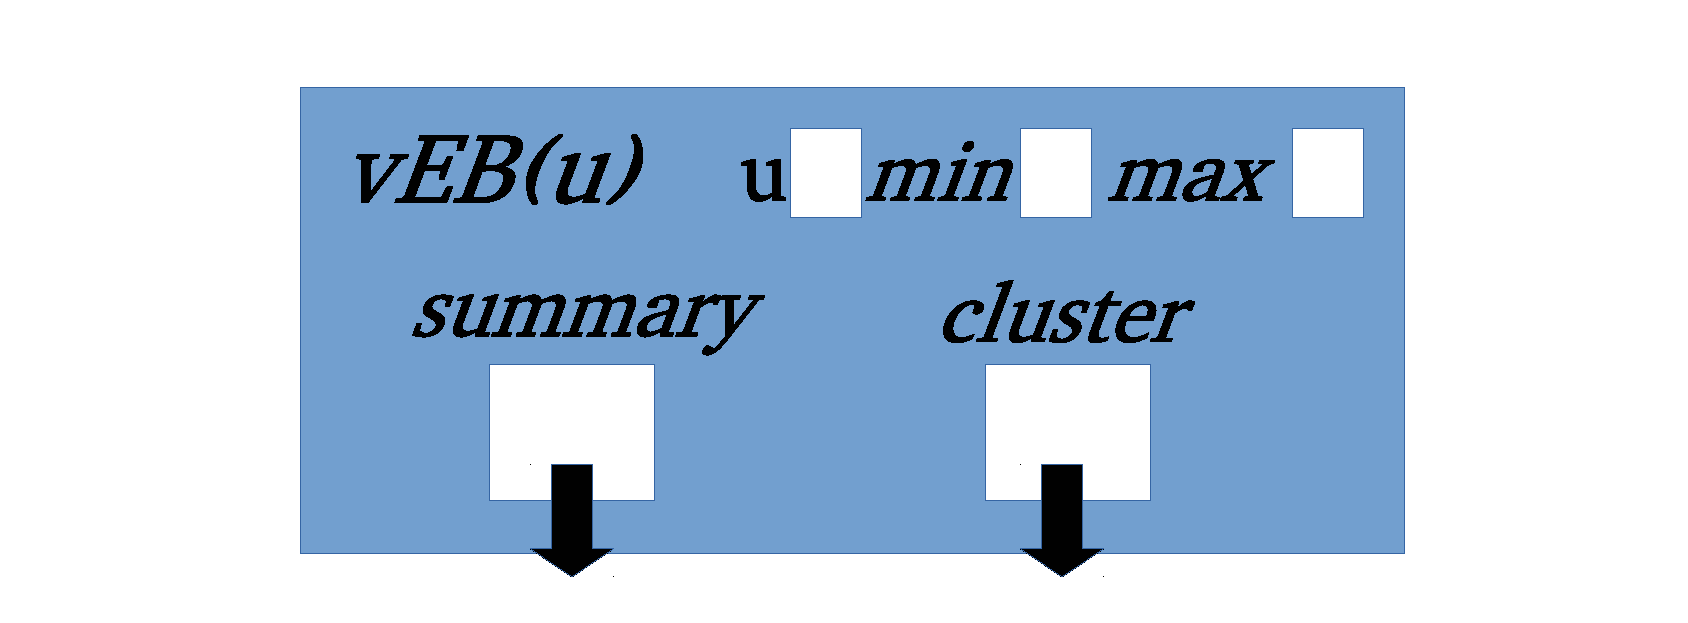
\includegraphics[width=\textwidth]{veb_node.eps}
\end{frame}

\begin{frame}\frametitle{謎木の特徴}
\begin{itemize}
\item 謎木では$cluster$が持つ要素が$\sqrt[\downarrow]{u}$となってしまう
\begin{itemize} \item 要素をそのまま格納したら再帰的に処理出来ない! \end{itemize}
\item $cluster$に処理を投げるときに, 引数で渡す$e$を$\sqrt[\downarrow]{u}$で割った余りにする
\item 復元するときは, $cluster\mbox{のインデクス}\times \sqrt[\downarrow]{u} + e\, mod \sqrt[\downarrow]{u}$とする
\end{itemize}
\end{frame}

\begin{frame}\frametitle{操作\; member(e)}
\begin{columns}
\begin{column}{0.4\textwidth}
\begin{itemize}
\item 自身が空であれば, $false$を返す
\item $min$か$max$に$e$があれば, $true$を返す
\item $summary$に$e$が格納されている$cluster$に要素がなければ$false$を返す
\item $cluster.member(e\, mod \sqrt[\downarrow]{u})$を返す
\end{itemize}
\end{column}
\begin{column}{0.59\textwidth}
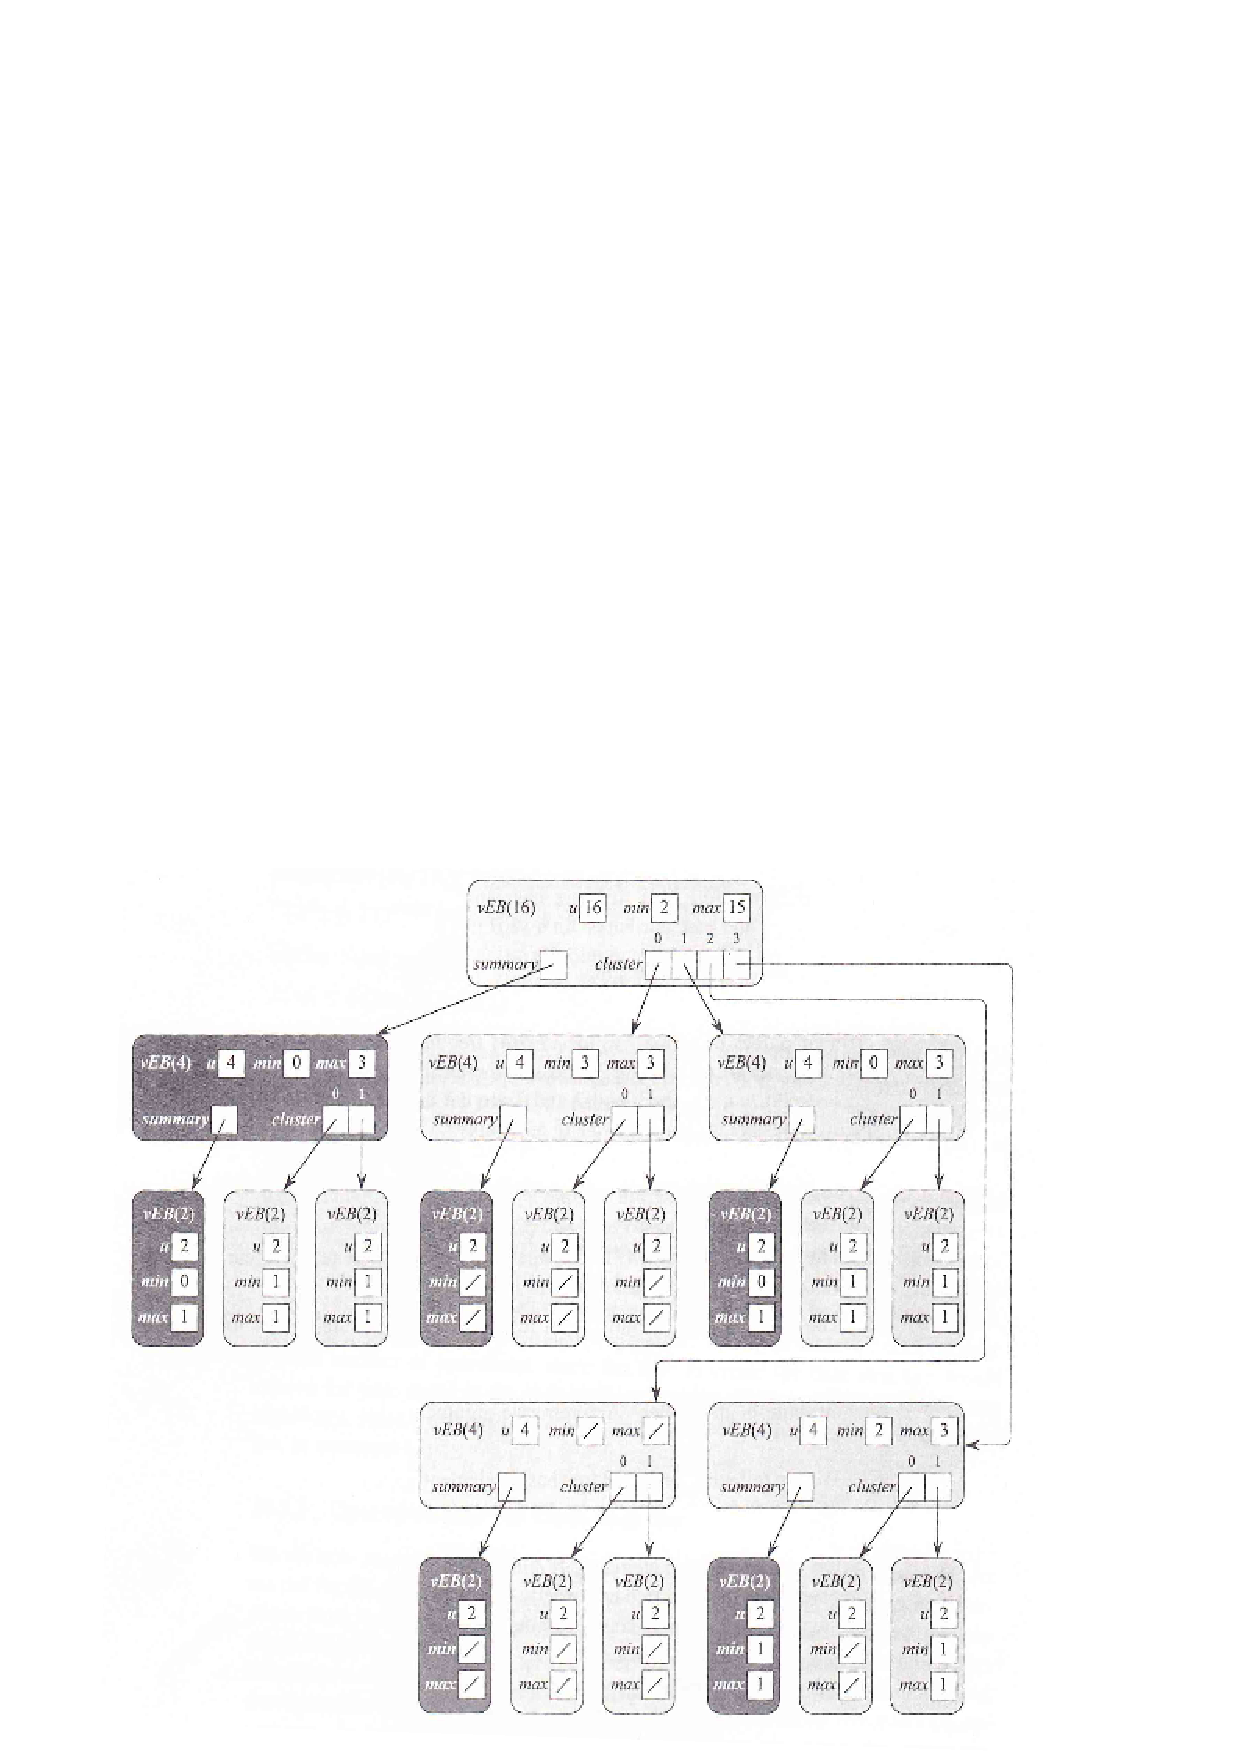
\includegraphics[width=\textwidth]{veb_fig.png}
\end{column}
\end{columns}
\end{frame}

\begin{frame}\frametitle{操作\; successor(e)}
\begin{itemize}
\item $e$が$min$より小さければ, $min$を返す
\item $\frac{e}{\sqrt[\downarrow]{u}}$番目の$cluster$の$max$が$e\,mod \sqrt[\downarrow]{u}$より小さければ,\\
	$cluster[\sqrt[\uparrow]{u}].successor(e\,mod \sqrt[\downarrow]{u})$を呼ぶ
\item そうでないなら, $summary.successor(\frac{e}{\sqrt[\downarrow]{u}})$を呼び, $e$が格納される$cluster$の次に要素を持つ$cluster$を見つける\\
	その$cluster$の$min()$を呼び, その$cluster$の持つ要素の最小値を返す
\end{itemize}
$predcessor(e)$も同様に処理する
\end{frame}

\begin{frame}\frametitle{操作\; insert(e)}
\begin{itemize}
\item 自身が空であれば, $min$と$max$を$e$に更新して終了
\item $e$が$min$より小さければ, \\ $min$と$e$の値を入れ替えて処理を続ける
\item $\frac{e}{\sqrt[\downarrow]{u}}$番目の$cluster$に要素がなければ, \\ $summary$に$\frac{e}{\sqrt[\downarrow]{u}}$を挿入し処理を続ける
\item $\frac{e}{\sqrt[\downarrow]{u}}$番目の$cluster$に$e\, mod \sqrt[\downarrow]{u}$を挿入する
\end{itemize}
\end{frame}

\begin{frame}\frametitle{操作\; delete(e)}
\begin{itemize}
\item 自身が要素を1つしか持たない($min$と$max$が同じ値)ならば, $min$と$max$の値を削除して処理を終える
\item そうでなく$u$が$2$のとき, 最小値と最大値を自分以外の数字に変える
\item そうでなく$e$が$min$と等しければ, $min$を$summary.min()$で得られた位置の$cluster$の最小値を, \alert{$e$}と$min$に代入し処理を続ける
\item $cluster[\frac{e}{\sqrt[\downarrow]{u}}].delete(e\, mod \sqrt[\downarrow]{u}$を呼び, 処理を続ける
\item $cluster[\frac{e}{\sqrt[\downarrow]{u}}]$が要素を持たないなら, \\
	\begin{itemize} \item $summary.delete(\frac{e}{\sqrt[\downarrow]{u}})$を呼ぶ
					\item $e$が$max$と等しければ, $summary.max()$で一番大きな要素を持つ$cluster$をみつけ, $max$をその要素と入れ替える\end{itemize}
\item そうでなく$e$が$max$と等しければ, $e$が格納されるはずの$cluster$の持つ最大値を$max$に代入する
\end{itemize}
\end{frame}

\begin{frame}\frametitle{計算量}
\begin{itemize}
\item \structure{空間計算量}
\par \hspace{1em} 各ノードは謎木ノード($u \; mod\sqrt[\downarrow]{u}$)へのポインタを$\frac{u}{\sqrt[\downarrow]{u}}+1$個持つノードの合計数は$2\times u$以下なので, $O(u)$
\begin{itemize} \item \onslide+<2->{\alert{\large{ダメ!}}}\end{itemize}
\item \structure{時間計算量}
\begin{itemize}
\item $min(), max()$は$O(1)$
\item $successor(e), predcessor(e), insert(e), delete(e)$は, $summary, cluster$両方に対し再帰的に関数を呼ぶ\\
木の高さは両方共$loglog(e)$以下なので時間計算量は$O(loglogu)$
\end{itemize}
\begin{itemize} \item \onslide+<2->{\structure{\large{はやい!}}}\end{itemize}
\end{itemize}
\end{frame}

\begin{frame}\frametitle{計算量}
\begin{itemize}
\item 競プロで使うならMLE
\item 要素を持たないノードが多すぎる
\item 本当に全てのノードを持つ必要があるか?
\pause
\item \large{必要ない!}
\item 空のノードにアクセスするのは$insert(e)$のときのみ!
\end{itemize}
\begin{block}{改善策}
空のノードに挿入するときに領域確保してみよう!
\end{block}
\end{frame}

\section{実装例}
\begin{frame}\frametitle{実装例\; メンバ変数}
\begin{columns}
\begin{column}{0.39\textwidth}
\begin{itemize}
\item c++で実装する際は$NULL$は数値なので要素を持たないことを保持するには, 工夫が必要
\item 今回は$max < min$として実装した
\item $u$は$2^k$となるような値なので$k$をメンバ変数として保持する
\end{itemize}
\end{column}
\begin{column}{0.6\textwidth}
\includegraphics[width=\textwidth]{veb_field.png}
\end{column}
\end{columns}
\end{frame}

\begin{frame}\frametitle{実装例\; $min(), max(), member(e)$}
\begin{columns}
\begin{column}{0.39\textwidth}
\begin{itemize}
\item $cluster$や$summary$への操作で, $\frac{e}{\sqrt[\downarrow]{u}}$などの値をよく使うため, 関数を用意
\end{itemize}
\end{column}
\begin{column}{0.6\textwidth}
\includegraphics[width=\textwidth]{veb_member.png}
\end{column}
\end{columns}
\end{frame}

\begin{frame}\frametitle{実装例\; $successor(e)$, $predcessor(e)$}
\begin{columns}[T]
\begin{column}{0.49\textwidth}
\includegraphics[width=\textwidth]{veb_succ.png}
\end{column}
\begin{column}{0.5\textwidth}
\includegraphics[width=\textwidth]{veb_pred.png}
\end{column}
\end{columns}
\end{frame}

\begin{frame}\frametitle{実装例\; $insert(e)$}
\begin{columns}
\begin{column}{0.39\textwidth}
\begin{itemize}
\item $empty-insert(e)$は$min\_$と$max\_$に$e$を代入している
\item $insert$時に格納する$cluster$を確保していなかったら新たに領域を確保する
\item $summary$も同様
\end{itemize}
\end{column}
\begin{column}{0.6\textwidth}
\includegraphics[width=\textwidth]{veb_ins.png}
\end{column}
\end{columns}
\end{frame}

\begin{frame}\frametitle{実装例\; $delete(e)$}
\begin{columns}
\begin{column}{0.49\textwidth}
\begin{itemize}
\item とある事情で関数名は$erase(e)$に
\item $cluster$が要素を持たなくなったら領域を解放している
\item $summary$も同様
\end{itemize}
\includegraphics[width=\textwidth]{veb_del0.png}
\end{column}
\begin{column}{0.5\textwidth}
\includegraphics[width=\textwidth]{veb_del1.png}
\end{column}
\end{columns}
\end{frame}

\section{性能評価}
\begin{frame}{性能評価}
以下の問題で評価
\begin{exampleblock}{Set: Range Search}
整数の集合$S$に対し以下の操作を行うこと. ただし, 集合$S$は要素の重複を許さない
\begin{itemize}
\item $insert(x)$: $S$に整数$x$を挿入する. さらに, 挿入直後の集合$S$の要素数を報告する
\item $find(x)$: $S$に含まれる$x$の数を報告する($0$または$1$)
\item $delete(x)$: $S$から$x$を削除する
\item $dump(L,R)$: $L$以上$R$以下である要素を順番に出力する
\end{itemize}
\small{出典: Aizu Online Judge ITP2\_7\_C}
\end{exampleblock}
\end{frame}

\begin{frame}{性能評価}
\begin{block}{}
\begin{center}
\begin{tabular}{|l|ll|}\hline
 & 実行時間 & メモリ使用量 \\\hline
std::set & 1.23s & 12368KB \\
謎木 & \alert<2->{1.38s} & \alert<3->{80136KB}\\\hline
\end{tabular}
\end{center}
\end{block}
\begin{itemize}
\pause
\item \LARGE{\alert{遅い!}}
\pause
\item \LARGE{\alert{重い!}}
\end{itemize}
\end{frame}

\begin{frame}{性能評価}
\begin{itemize}
\item なぜ処理に時間がかかるのか
\pause
\begin{itemize}
\item ノード作成時の領域確保がネック
\item 謎木ノード(2)が高頻度で領域確保, 解放が行われている可能性がある
\end{itemize}
\item 改善策は?
\pause
\item ノードを途中で切ってビット演算に切り替える
\pause
\item 予めメモリを確保しておいて, 各ノードに割り当てる
\begin{itemize} \item やってみたけどやり方が悪かったのかむしろ遅くなった \end{itemize}
\end{itemize}
\end{frame}

\section{まとめ}
\begin{frame}\frametitle{まとめ}
\begin{itemize}
\item 謎木は各種操作$O(loglogu)$で実行可能なデータ構造
\item ノードの持つ情報を$summary,cluster$が再帰的に保持する
\item 実装はデバッグがとても大変
\item \alert{競プロじゃ使わないかも}
\begin{itemize}\item 自分はこの実装をもっと高速化でもしないと使う気になれない \end{itemize}
\end{itemize}
\end{frame}


\end{document}
